% ----------------------------------------------------------------------------
% CONSTRUTOR E DESTRUTOR
% ----------------------------------------------------------------------------
\chapter{Construtor e destrutor}

\example{
\begin{itemize}
\item \texttt{example02.c}
\item \texttt{example09.c}
\end{itemize}
}

Um objeto em PD pode precisar de determinados parâmetros para ser iniciado.
Por exemplo, para criar um oscilador é necessário passar para este objeto a
frequência que o mesmo irá funcionar.
Assim, o objeto recebe um parâmetro como, por exemplo, [osc~ 440].
Para receber parâmetros na criação de um objeto é necessário informar o PD do mesmo.
Para isto, é necessário tanto informar os parâmetros na definição da classe quanto
definir corretamente a assinatura da função do construtor.
Estes parâmetros são ilustrados abaixo.

\begin{figure}[h!]
	\centering
	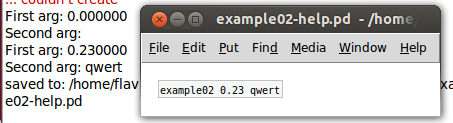
\includegraphics[scale=\Mysize]{example2}
	\caption{External recebendo parâmetros. Note a tela de saída no fundo da imagem.}
\end{figure}


% -----+-----+-----+-----+-----+-----+-----+-----+-----+-----+-----+-----+-----+
%      |     |     |     |     |     |     |     |     |     |     |     |     |
% -----+-----+-----+-----+-----+-----+-----+-----+-----+-----+-----+-----+-----+
\section{Tipos de parâmetros}

Os tipos de parâmetros aceitos para o construtor com checagem de tipo são:
\begin{itemize}
   \item \texttt{A\_DEFSYMBOL} para Strings
   \item \texttt{A\_DEFFLOAT} para números
\end{itemize}

Por questões de implementação, o PD pode verificar apenas 5 parâmetros com tipo.
Para passar mais parâmetros ao construtor é necessário utilizar um outro tipo
de parâmetro:

\begin{itemize}
   \item \texttt{A\_GIMME} para qualquer tipo de parâmetro
\end{itemize}

Caso este tipo seja utilizado, o construtor deverá receber uma lista de átomos
de tamanhos e tipos arbitrários e não faz a verificação de tipos.

A assinatura do construtor para receber ester parâmetros são:

\begin{lstlisting}[caption=Assinatura do construtor]
void *myclassnew(void) // Construtor sem parametros
void *myclassnew(t_symbol *arg)  // Para parametro tipo A_DEFSYMBOL
void *myclassnew(tfloatarg arg) // Para parametro tipo A_DEFFLOAT
void *myclass_new(t_symbol *s , int argc , t_atom * argv) // Para A_GIMME
\end{lstlisting}

% -----+-----+-----+-----+-----+-----+-----+-----+-----+-----+-----+-----+-----+
%      |     |     |     |     |     |     |     |     |     |     |     |     |
% -----+-----+-----+-----+-----+-----+-----+-----+-----+-----+-----+-----+-----+
\section{Construtor}

Parâmetros de inicialização no construtor podem permitir que inicializemos o
external com determinados valores. Isto é feito definindo os parâmetros no
métodos \texttt{class\_new()} quanto na definição da função construtora. (Veja o
exemplo02).

\begin{lstlisting}[caption=Passagem de parâmetro para o construtor]
// Constructos of the class
void * example02_new(t_floatarg arg1, t_symbol * arg2) {
    t_example02 *x = (t_example02 *) pd_new(example02_class);
    post("First arg: %f", arg1);
    post("Second arg: %s", arg2->s_name);
    return (void *) x;
}

void example02_setup(void) {
    example02_class = class_new(gensym("example02"),
            (t_newmethod) example02_new, // Constructor
            0,
            sizeof (t_example02),
            CLASS_NOINLET,
            A_DEFFLOAT, // First Constructor parameter
            A_DEFSYMBOL, // Second Constructor parameter
            0);
}
\end{lstlisting}

Notem que os parâmetros são definidos com um tipo e são recebidos com outro.
Como explicado na seção \ref{sec:mensagens}, todos os dados que não
correspondem a sinais de áudio são transmitidos como mensagens, compostas de
átomos.
Para ver os tipos de átomo que podem ser utilizados na passagem de parâmetros,
veja a seção \ref{sec:atomos}.

Para aceitar qualquer tipo de átomo na passagem de um parâmetro específico,
utilize o tipo de átomo \texttt{A\_GIMME} (veja o exemplo09).

\begin{lstlisting}[caption=Objeto que recebe qualquer tipo de parâmetro]
// Constructor of the class
void * example09_new(t_symbol *s, int argc, t_atom * argv) {
   t_example09 *x = (t_example09 *) pd_new(example09_class);
   post("%d parameters received",argc);
   return (void *) x;
}

void example09_setup(void) {
   example09_class = class_new(gensym("example09"),
     (t_newmethod) example09_new, // Constructor
     (t_method) example09_destroy, // Destructor
     sizeof (t_example09),
     CLASS_NOINLET,
     A_GIMME, // Allows various parameters
     0); // LAST argument is ALWAYS zero
}
\end{lstlisting}

Quando utilizamos o tipo de átomo \texttt{A\_GIMME} o método construtor
funciona como uma função \texttt{main()} em C: ela recebe os parâmetros
\texttt{argc}, que indica o número de átomos na lista, e \texttt{*argv}, que
aponta para a lista de átomos de fato. Veja o exemplo na figura
\ref{fig:construtor-parametros}.

\begin{figure}[h!]
\centering
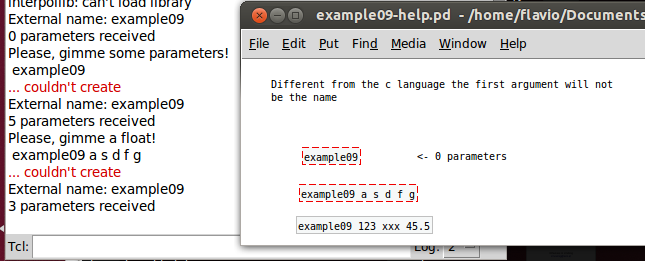
\includegraphics[scale=\Mysize]{example9}
\caption{Diferente da linguagem C, o primeiro parâmetro não é o nome do external.}
\label{fig:construtor-parametros}
\end{figure}

Neste caso, diferentemente da função main na linguagem C, o primeiro parâmetro
não é o nome do external.
O nome do external é o primeiro parâmetro recebido pela função, em nosso exemplo,
``t\_symbol *s''.

% -----+-----+-----+-----+-----+-----+-----+-----+-----+-----+-----+-----+-----+
%      |     |     |     |     |     |     |     |     |     |     |     |     |
% -----+-----+-----+-----+-----+-----+-----+-----+-----+-----+-----+-----+-----+
\section{Validando parâmetros no construtor}

Note que o Pure Data não obriga que o usuário passe parâmetros para o objeto.
Todo construtor, independentemente de como ele está definido, aceita
sua instanciação vazia.
Cabe ao programador verificar se os parâmetros recebidos são em quantidade,
tipo e valor esperado e, caso não seja, abortar a construção do objeto e não
retornar sua instância.

\begin{lstlisting}[caption=Validando parâmetros na construção de um objeto]
// Constructor of the class
void * example09_new(t_symbol *s, int argc, t_atom * argv) {
   t_example09 *x = (t_example09 *) pd_new(example09_class);
   post("External name: %s", s->s_name);
   post("%d parameters received",argc);
   if(argc < 1){
      post("Please, gimme some parameters!");
      return NULL;
   }
   if(argv[0]->a_type != A_FLOAT{
      post("Gimme a float!");
      return NULL;
   }
   return (void *) x;
}
\end{lstlisting}

Como podemos verificar no exemplo código acima, caso não seja passado um parâmetro
do tipo float para o example09 o mesmo não irá retornar uma instância do objeto
e apresentará a mensagem de que parâmetros devem ser passado ao objeto.

% -----+-----+-----+-----+-----+-----+-----+-----+-----+-----+-----+-----+-----+
%      |     |     |     |     |     |     |     |     |     |     |     |     |
% -----+-----+-----+-----+-----+-----+-----+-----+-----+-----+-----+-----+-----+
\section{Outras tarefas para o construtor}

Como deve-se saber, não é aconselhável alocar memória durante o bloco de
processamento de sinais quando trabalhamos com processamento em tempo real.
Por esta razão, é aconselhável alocar a memória de variáveis que iremos utilizar
em nosso \external no construtor.

Um exemplo de dados que deve ser alocado e instanciado no construtor seria uma
tabela seno para criar um oscilador por consulta a tabela.

\begin{lstlisting}[caption=Função para a alocação de memória]
void *getbytes(size_t nbytes);
\end{lstlisting}

A alocação de memória deve ser feita preferencialmente pela função \texttt{getbytes}.
Esta função utiliza internamente a função padrão \texttt{malloc} porém é portável
para os sistemas operacionais onde o PD funciona.

Outra tarefa que pode ser realizada pelo construtor é a criação de iolets
passivos.
Tal funcionalidade será coberta no próximo capítulo deste documento.

% -----+-----+-----+-----+-----+-----+-----+-----+-----+-----+-----+-----+-----+
%      |     |     |     |     |     |     |     |     |     |     |     |     |
% -----+-----+-----+-----+-----+-----+-----+-----+-----+-----+-----+-----+-----+
\section{Destrutor}

O destrutor de uma classe permite liberar alguma memória eventualmente alocada
pelo construtor ou por outras funções do \external (veja o exemplo 07).

\begin{lstlisting}[caption=Exemplo de destrutor]
// Destroy the object
void example09_destroy(t_example09 *x) {
  post("You say good bye and I say hello");
}

void example09_setup(void) {
   example09_class = class_new(gensym("example09"),
     (t_newmethod) example09_new, // Constructor
     (t_method) example09_destroy, // Destructor
     sizeof (t_example09),
     CLASS_NOINLET,
     A_GIMME, // Allows various parameters
     0); // LAST argument is ALWAYS zero
}
\end{lstlisting}

De maneira análoga a alocação de memória, o PD também disponibiliza uma função
portável para a liberação de memória.
A liberação da memória pode ser feita utilizando a função \texttt{freebytes()}
definida na API do Pure Data.
Tal função deve chamar internamente a função padrão \texttt{free} sendo, porém,
portável entre diferentes sistemas operacionais.

\begin{lstlisting}
void freebytes(void *x, size_t nbytes)
\end{lstlisting}
